\documentclass[letterpaper,11pt]{article}
\usepackage{graphicx}
\usepackage{listings}
\usepackage[super]{nth}
\usepackage[hyphens]{url}
\usepackage{hyperref}
\usepackage{amsmath}
\usepackage[makeroom]{cancel}
\usepackage[table]{xcolor}
\usepackage{comment}
\usepackage[space]{grffile}
\usepackage{csvsimple}

\newcommand*{\srcPath}{../src}%

\lstset{
	basicstyle=\footnotesize,
	breaklines=true,
}

\begin{document}

\begin{titlepage}

\begin{center}

\Huge{Assignment 4}

\Large{CS 532:  Introduction to Web Science}

\Large{Spring 2018}

\Large{Hrishi Gadkari}


\end{center}

\end{titlepage}

\newpage


% =================================
% First question
% =================================
\section*{1}


\subsection*{Question}

\begin{verbatim}
1.  1.  Determine if the friendship paradox holds for my Facebook
account.* Compute the mean, standard deviation, and median of the
number of friends that my friends have.  Create a graph of the
number of friends (y-axis) and the friends themselves, sorted by
number of friends (y-axis).  (The friends don't need to be labeled
on the x-axis: just f1, f2, f3, ... fn.)  Do include me in the graph
and label me accordingly.

* = This used to be more interesting when you could more easily download
your friend's friends data from Facebook.  Facebook now requires each
friend to approve this operation, effectively making it impossible.

I will upload a csv file of my 2014 friends list on the #assignment-4 slack channel
\end{verbatim}

\clearpage
\subsection*{Answer}

For the above problem, I wrote a script in R \cite{rdocref}. The script first extracts the  \textbf{FRIENDSCOUNT} column from the \textbf{friendscount.csv} file and sorts the values in ascending order. It then calculates the mean, median and standard deviation of Alexander Nwala’s Facebook friend counts as shown in Table \ref{table:q1summary}. The references used for this calculation were \cite{sortref} and \cite{statref}. 

\begin{table}[htb]
\centering
\begin{tabular}{ | l | l | l |}
\hline
\textbf{Mean} & \textbf{Standard Deviation} & \textbf{Median} \\
\hline
558.3176 & 571.784 & 397 \\
\hline
\end{tabular}
\caption{Mean, Standard Deviation and Median generated from R Script for Facebook friend counts}
\label{table:q1summary}
\end{table}


The R script as shown in Listing \ref{lst:q1face} is stored in \textbf{facebook.r} file 
The graph plotted as shown in Figure \ref{fig:q1facebookplot} tells us that Alexander Nwala has many friends which have higher friends count than him. This leads us to the conclusion that the friendship paradox holds for Alexander Nwala’s Facebook friends.

\lstinputlisting[frame=single,caption={R Script for generating plot of facebook friends},label=lst:q1face,captionpos=b,numbers=left,showspaces=false,showstringspaces=false,basicstyle=\footnotesize]{facebook.R}

\begin{figure}[h]
\centering
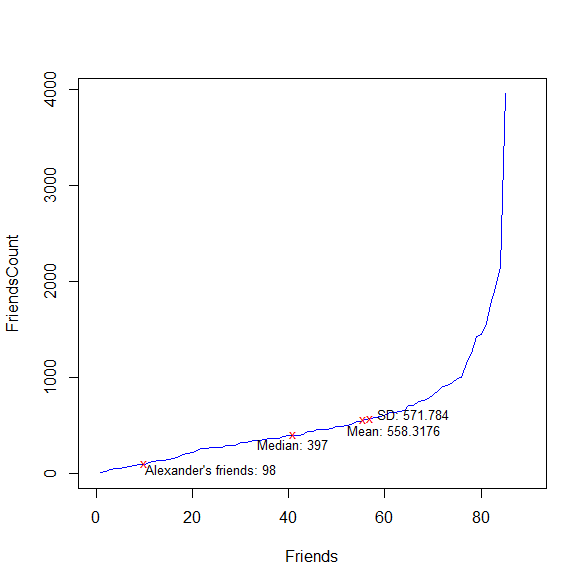
\includegraphics[scale=0.6]{facebook.png}
\caption{Plot of friends vs. friend counts}
\label{fig:q1facebookplot}
\end{figure}




\clearpage

% =================================
% Second question
% =================================

\section*{2}

\subsection*{Question}

\begin{verbatim}
2.  Determine if the friendship paradox holds for your Twitter account.
Since Twitter is a directed graph, use "followers" as value you measure
(i.e., "do your followers have more followers than you?").

Generate the same graph as in question #1, and calcuate the same 
mean, standard deviation, and median values.

For the Twitter 1.1 API to help gather this data, see:

https://developer.twitter.com/en/docs/accounts-and-users/follow-search-get-users/api-reference/get-followers-list

If you do not have followers on Twitter (or don't have more than 50),
then use my twitter account "acnwala".

\end{verbatim}

\clearpage
\subsection*{Answer}

Since my twitter account had followers less than 50, I user Alexander Nwala's twitter account. For the above problem I first went through the reference \cite{followerref}  mentioned in the question and came to know that in order to access the twitter followers API and get the followers list, I first need to register an application and get the keys and access tokens so as to access the API.
To solve the problem I wrote a script in Python 3.5 as shown in Listing \ref{lst:twitterpy}. The following dependencies were used:

\begin{itemize}
    \item import requests
    \item import tweepy
    \item from tweepy import OAuthHandler
    \item import csv
\end{itemize}

To get the followers list for the screen\_name: \textbf{acnwala} I went through the reference \cite{apiref} and used the tweepy.API() and  tweepy.Cursor() function. The program then gets the followers name and his followers counts one by one for Alexander Nwala’s Twitter followers and stores in \textbf{followers.csv} file.

\lstinputlisting[frame=single,caption={Python script for receiving twitter followers from Alexander Nwala's twitter},label=lst:twitterpy,captionpos=b,numbers=left,showspaces=false,showstringspaces=false,basicstyle=\footnotesize]{twitter.py}

To plot the graph I wrote a script in R \cite{rdocref}. The script first extracts the  \textbf{FollowersCount} column from the\textbf{ followers.csv} file and sorts the values in ascending order. It then calculates the mean, median and standard deviation of Alexander Nwala’s Twitter followers as shown in Table \ref{table:q2summary}. The references used for this calculation were \cite{sortref} and \cite{statref}. 


\begin{table}[htb]
\centering
\begin{tabular}{ | l | l | l |}
\hline
\textbf{Mean} & \textbf{Standard Deviation} & \textbf{Median} \\
\hline
2967.856 & 14353.86 & 274 \\
\hline
\end{tabular}
\caption{Mean, Standard Deviation and Median generated from R Script for Twitter follower counts}
\label{table:q2summary}
\end{table}

The R script as shown in Listing \ref{lst:q2process}  is stored in \textbf{tweetfor.r} file 


\lstinputlisting[frame=single,caption={R Script for generating plot of twitter followers},label=lst:q2process,captionpos=b,numbers=left,showspaces=false,showstringspaces=false,basicstyle=\footnotesize]{tweetfor.R}

The graph plotted as shown in Figure \ref{fig:q2followers} tells us that Alexander Nwala has many followers which have higher followers count than him. This leads us to the conclusion that the followers paradox holds for Alexander Nwala’s Twitter followers.

\begin{figure}[h]
\centering
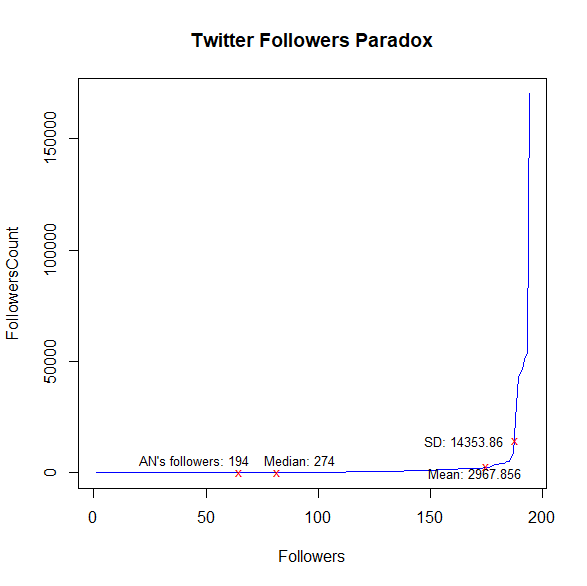
\includegraphics[scale=0.6]{twfr.png}
\caption{Plot of Alexander Nwala's  Twitter followers vs. follower counts}
\label{fig:q2followers}
\end{figure}





\clearpage

% =================================
% Third question
% =================================

\section*{3}

\subsection*{Question}

\begin{verbatim}
Extra credit, 1 point:

3.  Repeat question #1, but with your (or a specified) LinkedIn profile.

\end{verbatim}

\clearpage
\subsection*{Answer}

For the above problem I went through the github documentation \cite{linkref} of Linkedin API. I first installed the linkedin python library using  \textbf{pip install python3-linkedin}. I wrote a program in Python 3.5 as shown in Listing \ref{lst:q4script}. The following dependencies were used:

\begin{itemize}
    \item from linkedin import linkedin
\end{itemize}

The program gets the access tokens used for accessing the API and getting the profile for each user through OAuth by using id, secret key and return url. But after running the program it just returned the basic profile of my linked in profile giving the first name, last name and number of connections whereas access was denied for the get\_connections() and search\_profile(). I then googled and got to know that as of May 2017 \cite{permref}, Linked in have restricted its full API access and can be accessed only through special permissions. As per the Figure in  \ref{fig:q4link}, we can see that its returning just the number of connections.


\lstinputlisting[frame=single,caption={Python script for LinkedIn Profile API},label=lst:q4script,captionpos=b,numbers=left,showspaces=false,showstringspaces=false,basicstyle=\footnotesize]{link.py}

\begin{figure}[h]
\centering
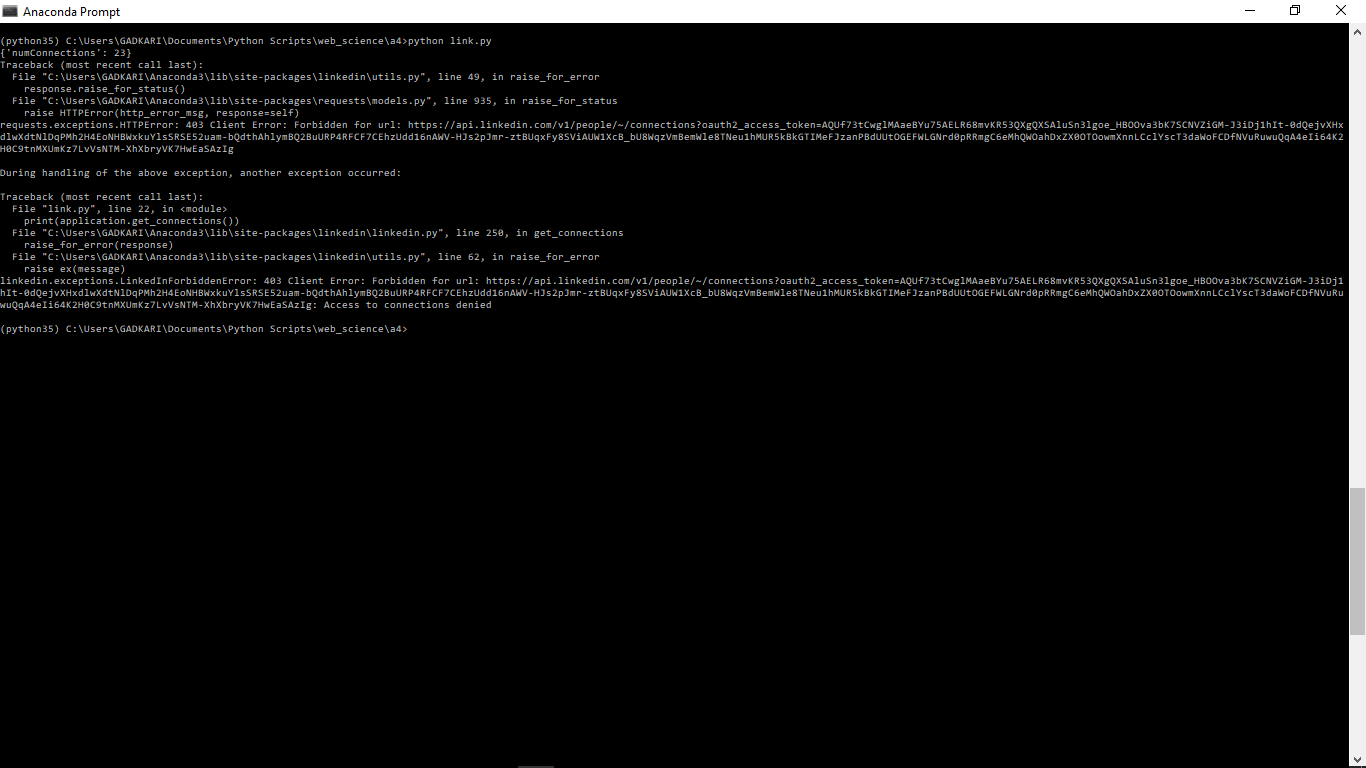
\includegraphics[scale=0.3]{linked.png}
\caption{Output for Linkedin API}
\label{fig:q4link}
\end{figure}



\clearpage




% =================================
% Fourth question
% =================================

\section*{4}

\subsection*{Question}

\begin{verbatim}
Extra credit, 3 points:

4.  Repeat question #2, but change "followers" to "following"?  In
other words, are the people I am following following more people?

For the Twitter 1.1 API to help gather this data, see:

https://developer.twitter.com/en/docs/accounts-and-users/follow-search-get-users/api-reference/get-
friends-list

\end{verbatim}

\clearpage
\subsection*{Answer}

 For the above problem, I repeated the same steps as mentioned in question 2.  I first went through the reference \cite{followingref}  mentioned in the question and came to know that in order to access the twitter's following/friends API and get the followings  list, I first need to register an application and get the keys and access tokens so as to access the API.
To solve the problem I wrote a script in Python 3.5 as shown in Listing \ref{lst:tweetfolpy}. The following dependencies were used:

\begin{itemize}
    \item import requests
    \item import tweepy
    \item from tweepy import OAuthHandler
    \item import csv
\end{itemize}

To get the followings list for the screen\_name: \textbf{acnwala} I went through the reference \cite{apiref} and used the tweepy.API() and  tweepy.Cursor() function. The program then gets the friends name and his following counts one by one for Alexander Nwala’s Twitter followings and stores in \textbf{following.csv} file.

\lstinputlisting[frame=single,caption={Python script for receiving twitter followers from Alexander Nwala's twitter},label=lst:tweetfolpy,captionpos=b,numbers=left,showspaces=false,showstringspaces=false,basicstyle=\footnotesize]{twitter.py}

To plot the graph I wrote a script in R \cite{rdocref}. The script first extracts the  \textbf{FollowingCount} column from the\textbf{ following.csv} file and sorts the values in ascending order. It then calculates the mean, median and standard deviation of Alexander Nwala’s Twitter friends as shown in Table \ref{table:q5summary}. The references used for this calculation were \cite{sortref} and \cite{statref}. 


\begin{table}[htb]
\centering
\begin{tabular}{ | l | l | l |}
\hline
\textbf{Mean} & \textbf{Standard Deviation} & \textbf{Median} \\
\hline
1032.158 & 1549.282 & 480.5 \\
\hline
\end{tabular}
\caption{Mean, Standard Deviation and Median generated from R Script for Twitter following counts}
\label{table:q5summary}
\end{table}

The R script as shown in Listing \ref{lst:follopy}  is stored in \textbf{tweetfol.r} file 


\lstinputlisting[frame=single,caption={R Script for generating plot of twitter followers},label=lst:follopy,captionpos=b,numbers=left,showspaces=false,showstringspaces=false,basicstyle=\footnotesize]{tweetfol.R}

The graph plotted as shown in Figure \ref{fig:q2follow} tells us that Alexander Nwala has many twitter friends which have higher followings count than him. This leads us to the conclusion that the following paradox holds for Alexander Nwala’s Twitter followers.

\begin{figure}[h]
\centering
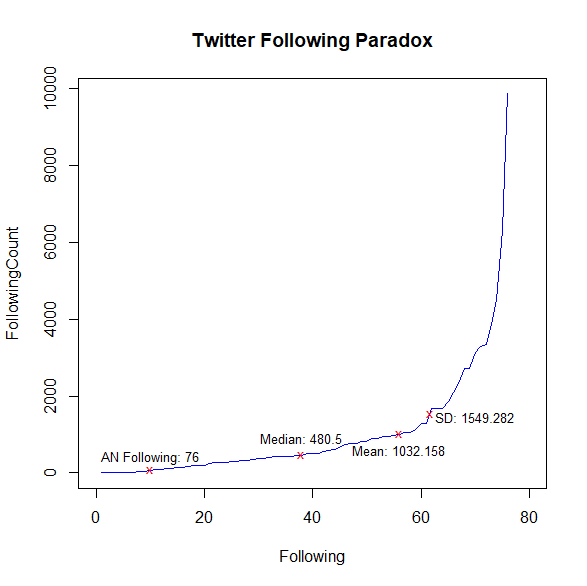
\includegraphics[scale=0.6]{twtfl.png}
\caption{Plot of Alexander Nwala's  Twitter followings vs. following counts}
\label{fig:q2follow}
\end{figure}


\clearpage

% =================================
% Bibliography
% =================================

\begin{thebibliography}{9}
\bibitem{followerref}
GET followers/list - Twitter Developers. ``Twitter.'' N.p., n.d. 27 February 2018.\url{https://developer.twitter.com/en/docs/accounts-and-users/follow-search-get-users/api-reference/get-followers-list}.
\bibitem{followingref}
GET friends/list - Twitter Developers. ``Twitter.'' N.p., n.d. 27 February 2018.\url{https://developer.twitter.com/en/docs/accounts-and-users/follow-search-get-users/api-reference/get-friends-list}.
\bibitem{rdocref}
Search all 14,436 CRAN, BioConductor and Github packages. ``R Documentation and manuals | R Documentation.''N.p., n.d. Web. 27 February 2018 \url{https://www.rdocumentation.org/}.
\bibitem{sortref}
base.``function | R Documentation''., n.d. Web. 27  February 2018. \url{https://www.rdocumentation.org/packages/base/versions/3.4.3/topics/sort}.
\bibitem{statref}
How to calculate mean, median, mode, std dev from distribution. ``r - How to calculate mean, median, mode, std dev from distribution - Cross Validated.''N.p., n.d. Web. 27 February 2018 \url{https://stats.stackexchange.com/questions/157661/how-to-calculate-mean-median-mode-std-dev-from-distribution}.
\bibitem{linkref}
Ozgur. ``Ozgur/python-linkedin.'', Github, 26 June 2015, n.d. Web. 27 February 2018 \url{https://github.com/ozgur/python-linkedin}.
\bibitem{apiref}
Get all followers and friends of a Twitter user. ``python - Get all followers and friends of a Twitter user - Code Review Stack Exchange.''N.p., n.d. Web. 27 February 2018 \url{https://codereview.stackexchange.com/questions/101905/get-all-followers-and-friends-of-a-twitter-user}.
\bibitem{permref}
Developer Program Transition | LinkedIn . ``LinkedIn Developers.''N.p., n.d. Web. 27 February 2018 \url{https://developer.linkedin.com/support/developer-program-transition}.

\end{thebibliography}

\end{document}